\section{Network Setup}
	
	The nature of this project is such that all client VMs need to be able to communicate with each other and the Index Server to send messages (\hyperlink{sec:client_ops}{operations}) and file segments.  We do not anticipate that a larger deployment of this system would warrant an exception to this assumption, since even if it were the case that multiple physical servers were running the client VMs in different locales, these servers should be networked such that the clients still view each other as though they were all connected to the same local network.
	
	\begin{figure}[th]
		\centering
		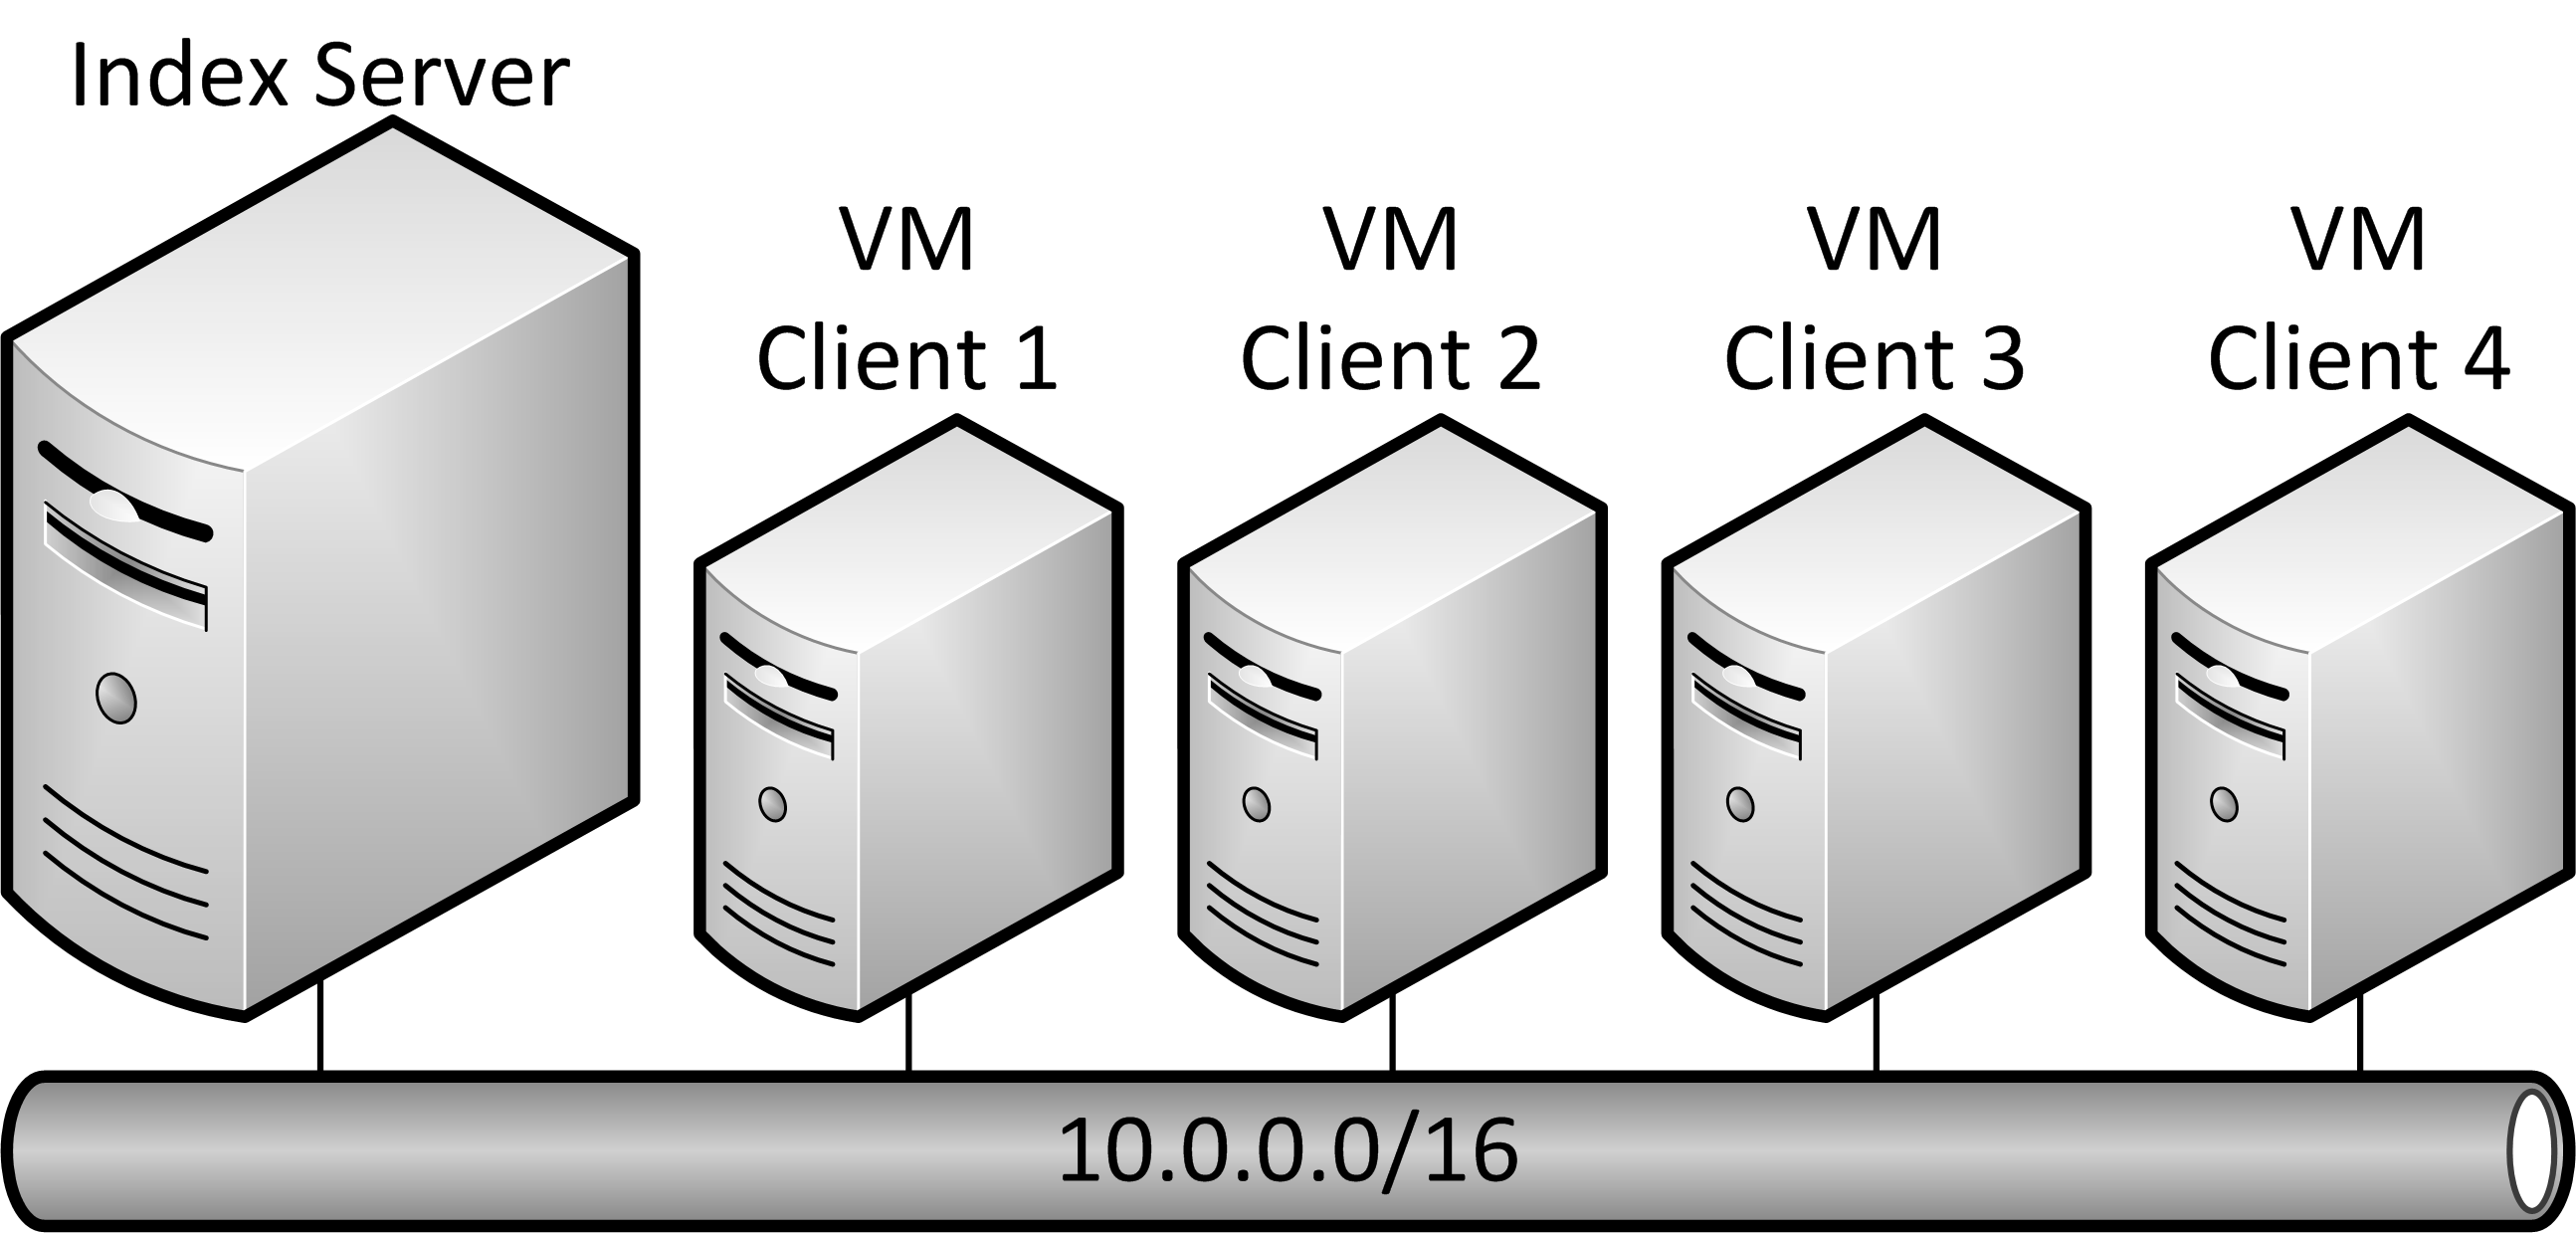
\includegraphics[scale=1]{figs/network_setup}
		\caption{The network consists of the Index Server and four virtual machines that can all communicate with each other on the 10.0.0.0/16 network to which they are connected.}
		\label{fig:network_setup}
	\end{figure}
	
	As illustrated in Figure~\ref{fig:network_setup}, the Index Server and all four of the client VMs are on the 10.0.0.0/16 network.  The IP addresses of the machines are as follows.
	
	\begin{itemize*}
		\item \textbf{Index Server:} 10.0.102.155
		\item \textbf{VM Client 1:} 10.0.102.154
		\item \textbf{VM Client 2:} 10.0.102.153
		\item \textbf{VM Client 3:} 10.0.102.152
		\item \textbf{VM Client 4:} 10.0.102.151
	\end{itemize*}
